\documentclass[a4paper,14pt]{extreport}
\usepackage[left=1.5cm,right=2cm,
    top=1.5cm,bottom=2cm,bindingoffset=0cm]{geometry}
\usepackage{scrextend}
\usepackage[T1,T2A]{fontenc}
\usepackage[utf8]{inputenc}
\usepackage[russian,ukrainian,english]{babel}
\usepackage{tabularx}
\linespread{1.5}
\usepackage{amssymb}
\usepackage{color}
\usepackage{amsmath}
\usepackage{mathrsfs}
\usepackage{listings}
\usepackage{graphicx}
\graphicspath{ {./images/} }
\usepackage{lipsum}
\usepackage{xcolor}
\usepackage{hyperref}
\usepackage{tcolorbox}
\usepackage{tikz}
\usepackage[framemethod=TikZ]{mdframed}
\usepackage{wrapfig,boxedminipage,lipsum}
\mdfdefinestyle{MyFrame}{%
linecolor=blue,outerlinewidth=2pt,roundcorner=20pt,innertopmargin=\baselineskip,innerbottommargin=\baselineskip,innerrightmargin=20pt,innerleftmargin=20pt,backgroundcolor=gray!50!white}
 \usepackage{csvsimple}
 \usepackage{supertabular}
\usepackage{pdflscape}
\usepackage{fancyvrb}
%\usepackage{comment}
\usepackage{array,tabularx}
\usepackage{colortbl}

\usepackage{varwidth}
\tcbuselibrary{skins}
\usepackage{fancybox}


\usepackage{tikz}
\usepackage[framemethod=TikZ]{mdframed}
\usepackage{xcolor}
\usetikzlibrary{calc}
\makeatletter
\newlength{\mylength}
\xdef\CircleFactor{1.1}
\setlength\mylength{\dimexpr\f@size pt}
\newsavebox{\mybox}
\newcommand*\circled[2][draw=blue]{\savebox\mybox{\vbox{\vphantom{WL1/}#1}}\setlength\mylength{\dimexpr\CircleFactor\dimexpr\ht\mybox+\dp\mybox\relax\relax}\tikzset{mystyle/.style={circle,#1,minimum height={\mylength}}}
\tikz[baseline=(char.base)]
\node[mystyle] (char) {#2};}
\makeatother

\definecolor{ggreen}{rgb}{0.4,1,0}
\definecolor{rred}{rgb}{1,0.1,0.1}
\definecolor{amber}{rgb}{1.0, 0.75, 0.0}
\definecolor{babyblue}{rgb}{0.54, 0.81, 0.94}
\definecolor{asparagus}{rgb}{0.53, 0.66, 0.42}
\definecolor{chartreuse}{rgb}{0.5, 1.0, 0.0}
\definecolor{darkorchid}{rgb}{0.6, 0.2, 0.8}

\usepackage{float}
\usepackage{wrapfig}
\usepackage{framed}
%for nice Code{
\lstdefinestyle{customc}{
  belowcaptionskip=1\baselineskip,
  breaklines=true,
  frame=L,
  xleftmargin=\parindent,
  language=C,
  showstringspaces=false,
  basicstyle=\small\ttfamily,
  keywordstyle=\bfseries\color{green!40!black},
  commentstyle=\itshape\color{purple!40!black},
  identifierstyle=\color{blue},
  stringstyle=\color{orange},
}
\lstset{escapechar=@,style=customc}
%}


\begin{document}
\pagecolor{white}

%----------------------------------------1
\newtcbox{\xmybox}[1][red]{on line, arc=7pt,colback=#1!10!white,colframe=#1!50!black, before upper={\rule[3pt] {0pt}{10pt}},boxrule=1pt,boxsep=0pt,left=6pt,right=6pt,top=2pt,bottom=2pt}

\begin{center}\xmybox[green]{Mnatsakanov Anton} \xmybox[amber]{DP-82} \xmybox[blue]{Variant №5}
\vspace{1cm}

\end{center}


\begin{center}Наведіть модельне представлення сегнетоелектрики.\end{center}

In general, ferroelectrics are a subclass of pyroelectrics in which the spontaneously polarized state is not stable enough and therefore quite labile (pliable). This condition can be changed by external influences: electric field, temperature change, mechanical pressure, etc.. 


\begin{figure}[h]
\center{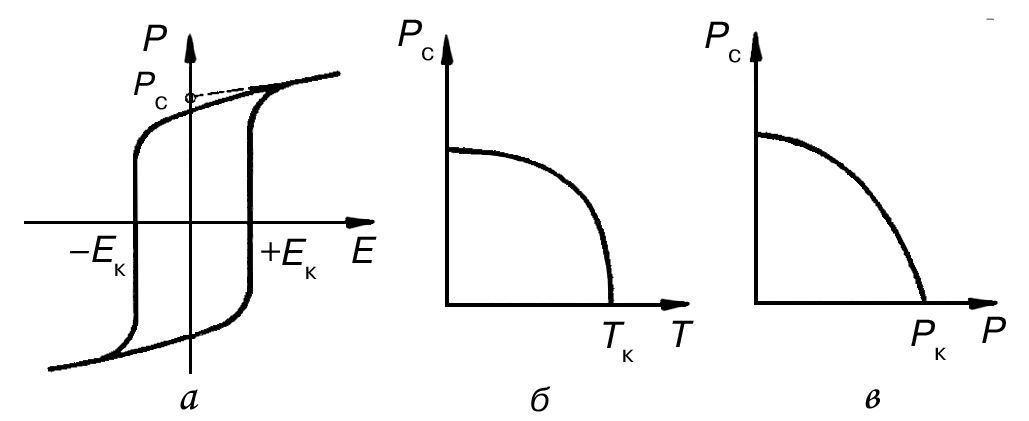
\includegraphics[width=0.7\linewidth]{1.png}}
\caption{dependence of the polarization P of ferroelectrics on the voltage
electric field (a) and spontaneous polarization of RS from temperature (b) and pressure (c) }
\label{ris1}
\end{figure}

For qualitative analysis, a one-dimensional ion chain is used as the simplest model. For analysis, we can use the energy decomposition U of a linear chain of ions into a series by the magnitude of the elastic displacements x:
\begin{equation}
U(x)  = \dfrac{1}{2} cx^2 + \dfrac{1}{2} bx^4 + ...
\end{equation}

To consider the polarization of ordinary ("linear") dielectrics, it suffices to confine oneself to the first term of this expansion: $ U (x) = \ dfrac {1} {2} cx ^ 2 $. To identify the role of anharmonicity, we can limit ourselves to a simple approximation, which takes into account, in addition to the quadratic term of energy decomposition with coefficient of elasticity c, the first anharmonic term with coefficient of anharmonicity b> 0. For simplification, it is assumed that ferroelectrics paraelectric) phase is centrosymmetric, while polar ferroelectric crystals are not centrosymmetric. \\

У разі переходу в спонтанно поляризований стан до розкладання в ряд функції U(х) додається лінійний за величиною спонтанного зміщення член Fx:
\begin{equation}
U(x)  = \dfrac{1}{2} cx^2 + \dfrac{1}{2} bx^4 -Fx,
\label{eq2}
\end{equation}
where x is the deformation and F is the strength of the internal (spontaneous) electric field.

The graphs of the function U (x) for the cases c> 0 and c <0 are shown in Fig.
\ref{ris2}



\begin{figure}[h]
\center{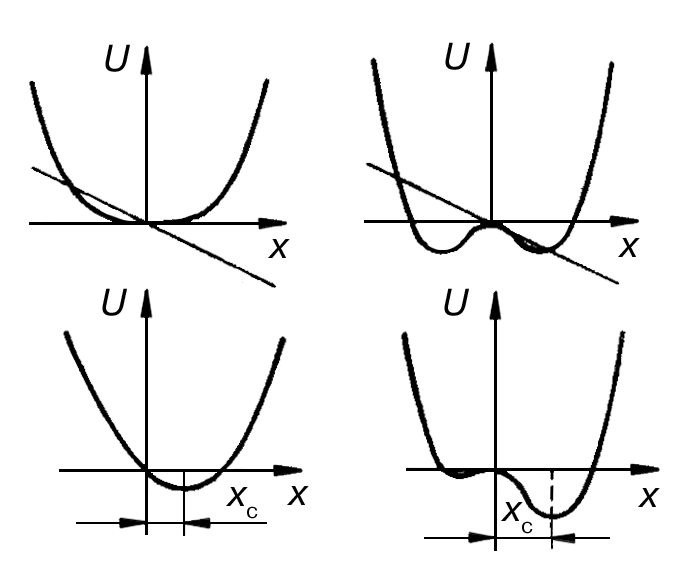
\includegraphics[width=0.7\linewidth]{2.png}}
\caption{Anharmonism and ferroelectrics: energy dependence of U "ferroeactive"
  ion from its localization x in the crystal lattice taking into account the linear
by the deformation of the contribution Fx, which causes the spontaneous deformation of $ x_c $}
\label{ris2}
\end{figure}




It is seen that below the Curie point there is a constant displacement xs, ie spontaneous deformation, at which the energy U (x) is minimal. Since the spontaneously polarized state at x = $ x_c $ is equilibrium, the total force acting on the charge system in this state is zero:
\begin{equation}
\dfrac{\partial U(x)}{\partial x}  =  0 \text{якщо } x = x_{c} \text{тобто } cx_{c}^2 + bx_{c}^4 - F = 0
\end{equation}
With spontaneous polarization is associated an electric field called
coercive field: $ F_ {c} = \ beta_ {c} $, where $ \ beta- $ Lorentz coefficient
$$
c x_{c}+b x_{c}^{3}-n q^{2} \beta x_{c}=0
$$
where the parameter $ _ {c} $ characterizes the "elasticity", a $ b- $ the parameter of anharmonism. This equation has the following three roots:
\begin{equation}
x_{1}=0 ; x_{2,3}= \dfrac{\sqrt{(\operatorname{nq2} \beta-c)}}{b}.
\label{eq3}
\end{equation}
Since a spontaneously polarized phase with spontaneous deformation $ x _ {\ mathrm {c}} \ neq 0 $ is considered, the first solution {} $ \ left (x_ {1} = 0 \ right) \ epsilon $ is lateral and below the point Curie is not realized.

An analysis of the other two solutions allows us to draw the following conclusions. First, the signs "$ \ pm $" mean two equal possible directions of spontaneous polarization, corresponding to two identical in absolute value, but different in the direction of the ion displacement: $ \ pm $ xs. This corresponds to two values ​​of $ \ pm $ Rs. Indeed, the spontaneous polarization of ferroelectrics in some parts of the crystal is directed in one direction, and in others - in the other (these areas with the same directional Pc are called domains).

Second, in crystals with a weakly pronounced anharmonicity, when b $ \ approx $ 0, spontaneous ion displacements are not possible at all. Thus, anharmonism is one of the defining properties of ferroelectric crystals.
Third, the equation \ ref {eq3} has real roots x2,3 only under the condition $ n q ^ 2 \ beta $> c (because the parameter b> 0). To find out the physical meaning of this important inequality - the conditions for the appearance of spontaneous polarization - we must multiply the left and right parts of the expression $ n q ^ 2 \ beta $> c by the deformation x:
\begin{equation}
n q^2 \beta x > c x
\end{equation}
The right-hand side of this inequality corresponds to the elastic force that counteracts the ferroelectric spontaneous shift. It by its nature corresponds to the repulsion of the electronic shells of ions and is an interaction that returns the nonpolar state. Therefore, in the left-hand side of inequality (8.6) the expression $ n q ^ 2 \ beta x $ has the dimension and content of the force called the leading interaction (which leads to ferroelectricity). Spontaneous polarization occurs in those crystals in which the leading interaction exceeds the opposing interaction.









\end{document}
